% !TeX root = ../main.tex

\chapter{LXeTPC与HPGe探测器的工作原理}

了解探测器的结构和信号产生过程对于信号测量和本底估计必不可少,
本章将以暗物质探测实验中的LXeTPC和HPGe探测器应用为基础,介绍两类探测器的工作原理,
并设计一种能够在地面反应堆附近运行的LXeTPC探测器及屏蔽体结构。

\section{LXeTPC的基本工作过程}

\begin{figure}
    \centering
    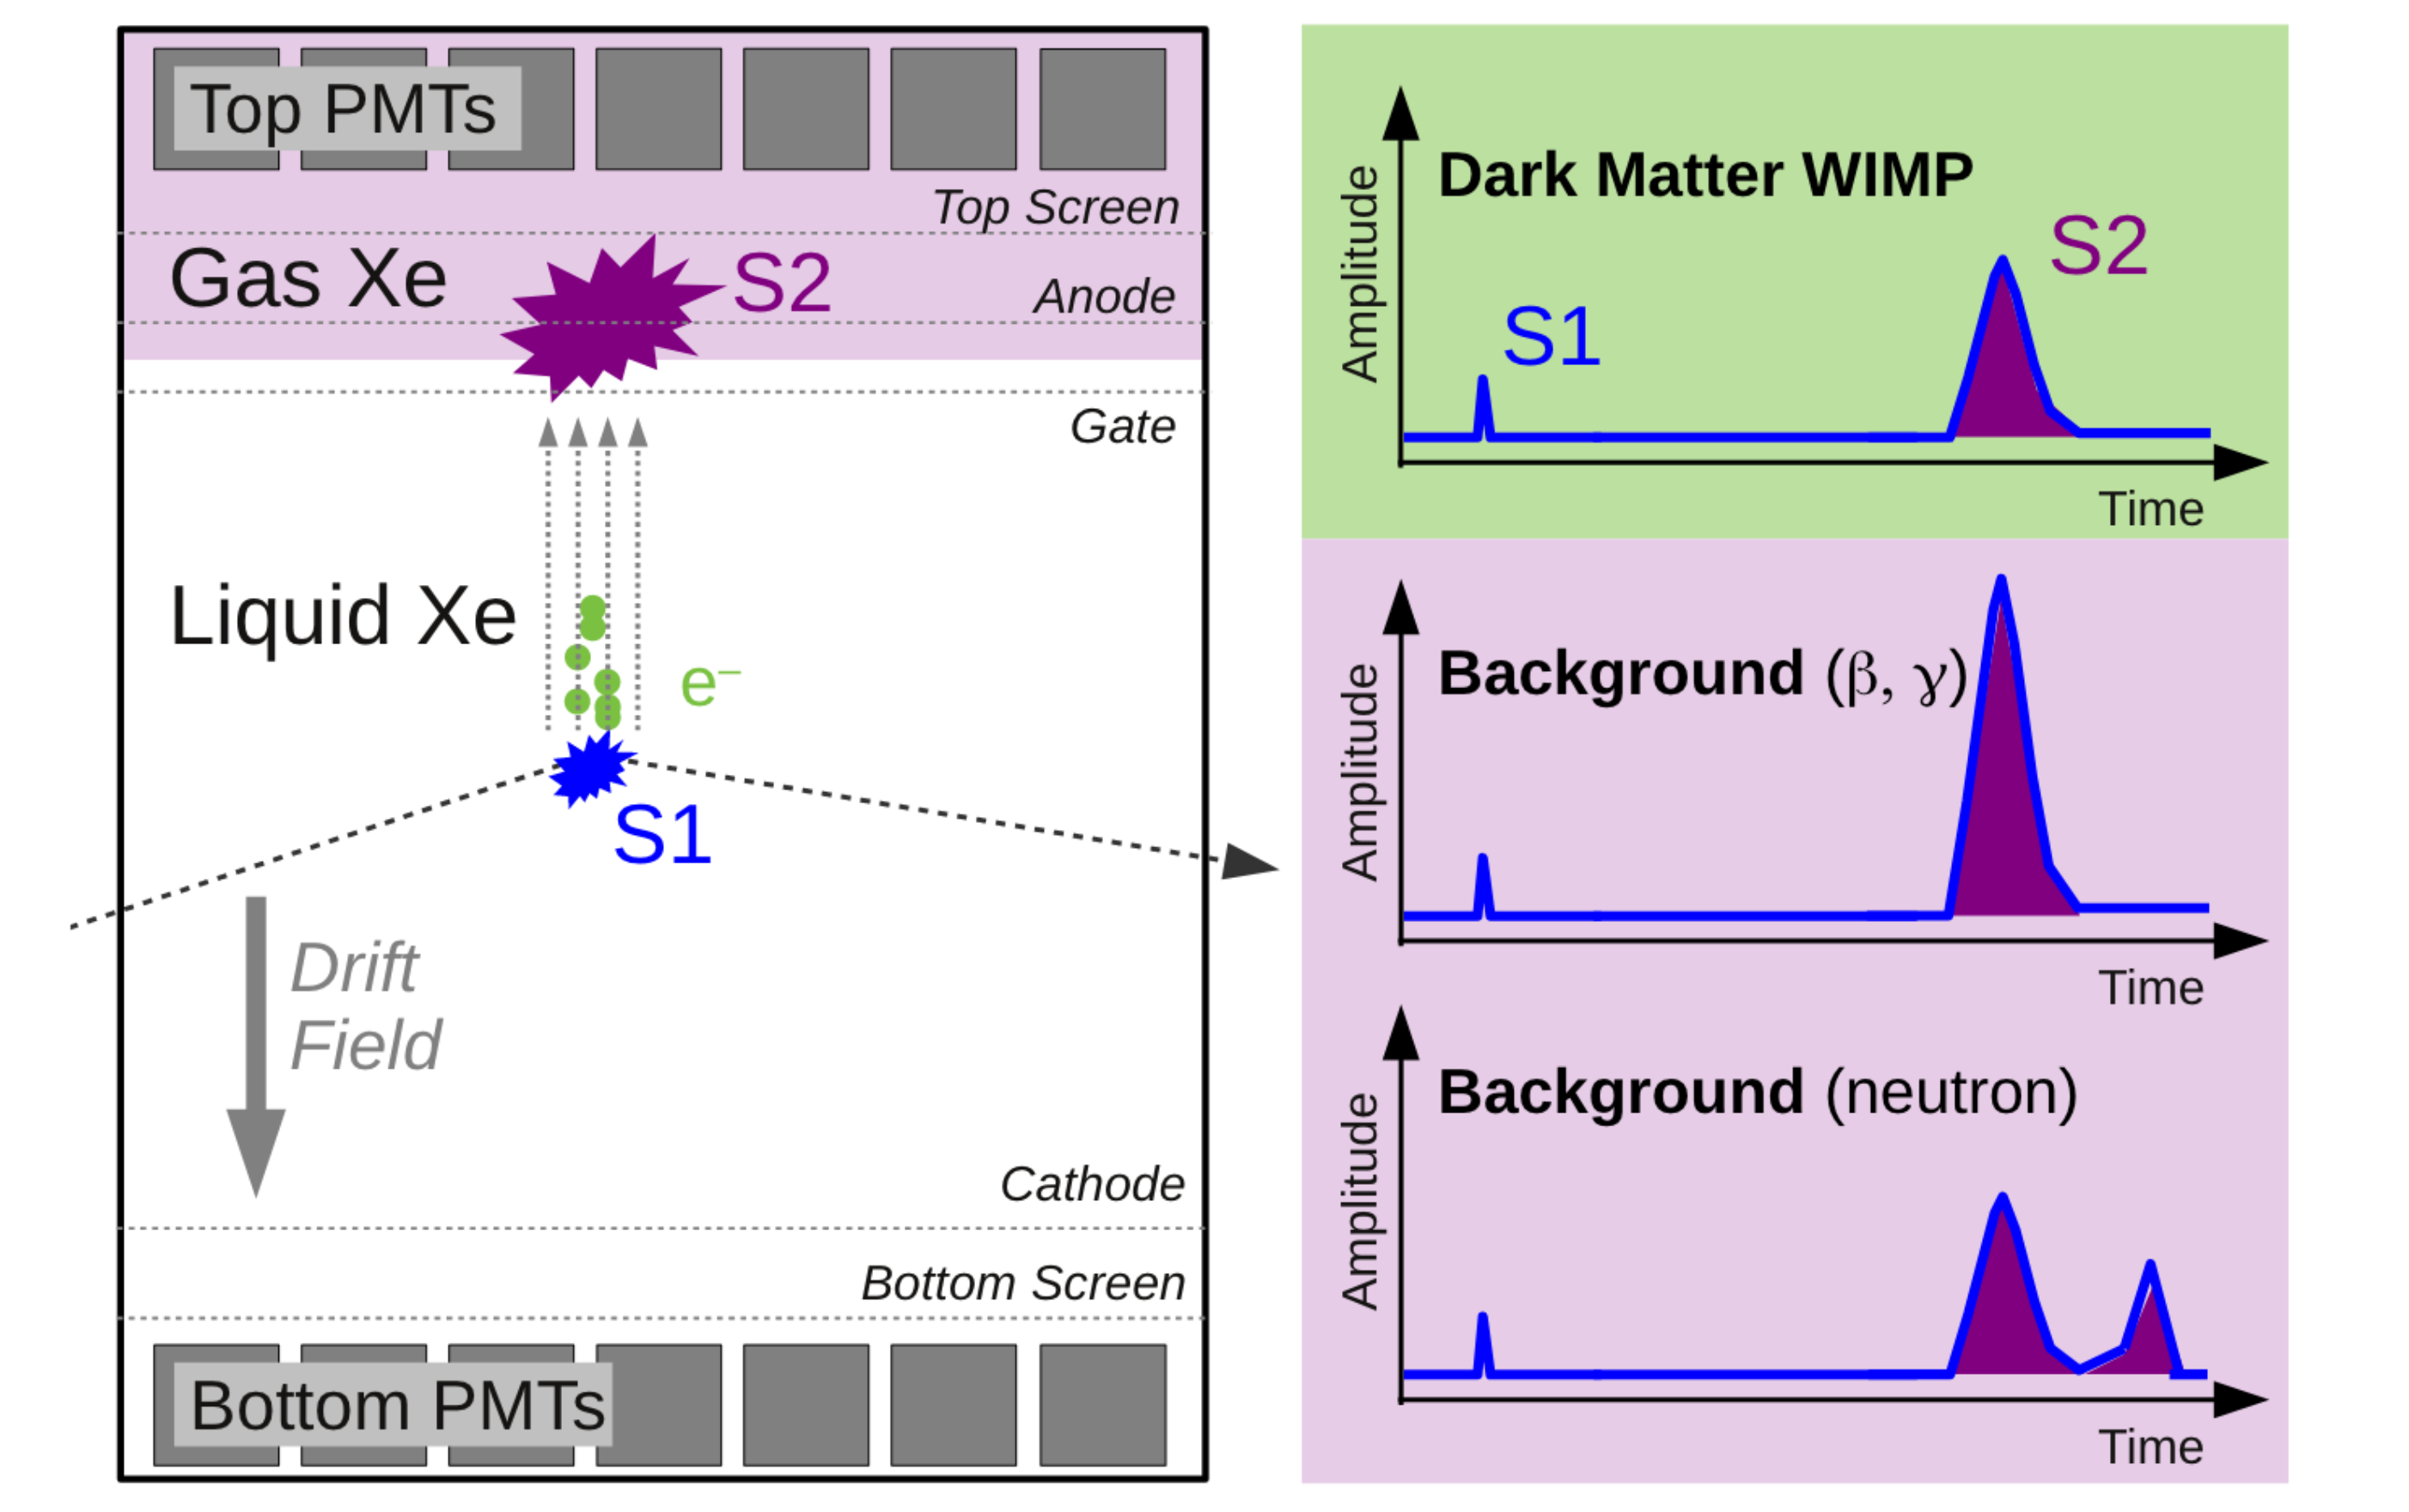
\includegraphics[width=0.7\linewidth]{figures/tpc_signals.png}
    \caption{\label{fig:tpc_principle} LXeTPC工作原理示意图。TPC的上下端安装有两组光电倍增管(photomultiplier tube, PMT)阵列。
    当入射粒子,如WIMP或中微子,撞击$\mathrm{Xe}$原子核,闪烁光信号将被PMT阵列探测到。一组TPC电极会建立几段纵向电场。
    能量沉积最终转化为电离电子的动能,在阴极(Cathode)和门电极(Gate)之间纵向电场的作用下,
    电子向上漂移并在门电极和阳极(Anode)之间产生正比闪烁光,该闪烁光也会被PMT阵列探测到。\cite{xenon_collaboration_xenon1t_2017}。}
\end{figure}

图\ref{fig:tpc_principle}简要呈现了LXeTPC的工作原理。圆柱形TPC分为上下气液两种相态,并安装5层电极。
从上至下,电极分别为上屏蔽(Top Screen),阳极,门电极,阴极和下屏蔽(Bottom Screen)。
上屏蔽和阳极在气氙中,其余三个电极浸泡在液氙中。
阴极和门电极之间建立均匀漂移电场,门电极和阳极之间有强电场,可以将液面下电子拉出。

入射的中子、中微子或WIMP携带能量与液氙中原子核碰撞,产生核反冲;
入射电子核$\gamma$光子与电子相互作用,相应地产生电子反冲(electronic recoil, ER)。

反冲能会激发或电离液氙,激发态的$\mathrm{Xe_2^*}$退激,
在灵敏体积中产生波长为178$\si{nm}$的闪烁光,称为$\mathrm{S1}$,闪烁光在液氙中传播,
经过一系列光学过程后被PMT阵列收集并在数据采集(data acquisition, DAQ)系统中被记录下来。
能量沉积也会产生电离信号,在漂移电场作用下,电子从阴极方向向门电极方向漂移,在门电极和阳极之间的电场中被拉出至液面,
并在气态氙中产生闪烁光,称为$\mathrm{S2}$。另外也有一部分能量沉积以热能形式耗散。
能量沉积产生光信号、电子信号和热能的比例由反冲的类型和能量决定,由此我们可以一定程度上区分电子反冲和核反冲信号。

探测器中事件的能量和位置重建对实现精确的信号探测及最终的物理目标是至关重要的。
事件发生的纵向位置 $z$可以通过$\mathrm{S1}$和$\mathrm{S2}$之间的时间差和电子漂移速度计算得出。
事件在TPC圆柱的上下表面投影位置可以通过顶部PMT阵列接收到的$\mathrm{S2}$图案通过位置重建算法得到。

\section{LXeTPC的响应模型}
\label{sec:basic_response}

液氙中有三种基本能量响应:热能耗散、氙原子激发和氙原子电离。LXeTPC一般不能探测热能。
液氙中的能量响应可以用NEST(the Noble Element Simulation Technique)模型描述\cite{szydagis_nest_2011,lenardo_global_2015}。
激发态的氙数目$N_{\mathrm{ex}}$和被电离的电子-氙离子对个数$N_i$之和为可探测的量子(quanta)数$N_q$,
$N_q$可以用于重建反冲能$\varepsilon $。在热能损失下,$N_q$服从二项分布:

\begin{align}
    \label{eq:N_q}
    N_q &\sim \mathrm{Binom}\left(\varepsilon /W,L\right)
\end{align}

其中$L$为Lindhard因子,用于描述热能损失的比例;
$W$是能量沉积产生一个激发态氙或电子-氙离子所需平均能量,
实验测得$W=13.7\pm0.2\si{eV}$\cite{szydagis_nest_2011}。
在电子反冲过程中,因为电子质量远小于氙原子核质量,所以以热能损失的能量可以忽略不计;
在核反冲过程中,反冲氙原子以弹性散射方式向其周围氙原子传递动能,Lindhard因子$L$取值为$0.1\sim0.2$。
$L$对电场大小和反冲能量的依赖关系可以由NEST模型描述。

激发-电离比$\langle N_{\mathrm{ex}}/N_i\rangle$反冲粒子对氙原子核的激发和电离截面有关。
对于电子反冲,这个值被认为是在0.06到0.20之间的常数。
对于核反冲,激发-电离比是沉积能量和灵敏体积内电场$F$的函数\cite{lenardo_global_2015}。
在$81\si{kV/cm}$电场下,$5-40\si{keV_{nr}}$的核反冲的激发-电离比在0.7到1.0之间。
$N_i$和$N_{\mathrm{ex}}$的涨落可以用二项分布描述:

\begin{align}
    \label{eq:N_iex}
    N_i &\sim \mathrm{Binom}\left(N_q,\frac{1}{1+\langle N_{\mathrm{ex}}/N_{i}\rangle}\right) \\
    N_{\mathrm{ex}} &= N_q - N_i
\end{align}

电离电子有一定的几率$1-r$从电子-离子对中逃逸,$r$被称为重组比例(\mbox{recombination} ratio)。

\begin{align}
    \label{eq:N_er}
    N_e &\sim \mathrm{Binom}\left(N_i,1-r\right) \\
    N_\gamma &= N_i - N_e + N_{\mathrm{ex}}
\end{align}

式\ref{eq:N_er}中,$N_\gamma$为激子推激以及电子-离子对重组放出的光子个数,$N_{e}$为逃逸的电子个数。
因为某些探测器效应,如电场不均匀性和某些内禀涨落\cite{lux_collaboration_tritium_2016},我们用正态分布来描述$r$:

\begin{align}
    \label{eq:r}
    r &\sim \mathrm{Gauss}\left(\langle r\rangle,\Delta r\right)
\end{align}

平均重组比例$\langle r\rangle$依赖于沉积能量大小和电场强弱,
其可以用Thomas-Imel(TI)箱模型描述\cite{thomas_recombination_1987}:

\begin{align}
    \label{eq:mr}
    \langle r\rangle &= 1 - \frac{\ln{\left(1+N_i\varsigma/4\right)}}{N_i\varsigma/4}
\end{align}

其中$\varsigma$是TI模型中的电场场强相关的参数。$\Delta r$描述了重组比例的涨落:

\begin{align}
    \label{eq:sr}
    \Delta r &= q_2\left(1-e^{-\varepsilon /q_3}\right)
\end{align}

平均的光子产额(light yield)$L_y=\langle N_\gamma\rangle/\varepsilon $和电子产额(ionization yield)$Q_y=\langle N_e\rangle/\varepsilon $定义为:

\begin{align}
    \label{eq:N_g}
    L_y &= \langle N_\gamma\rangle/\varepsilon  = \frac{1}{W}\frac{\langle r\rangle+\langle N_{\mathrm{ex}}/N_i\rangle}{1+\langle N_{\mathrm{ex}}/N_i\rangle} \\
    \label{eq:N_e}
    Q_y &= \langle N_e\rangle/\varepsilon  = \frac{1}{W}\frac{1-\langle r\rangle}{1+\langle N_{\mathrm{ex}}/N_i\rangle}
\end{align}

本文中将不细致讨论光子和电子产生的微观过程,而将光子产额$L_y$和电子产额$Q_y$作为带不确定度的参数。

\section{LXeTPC的探测器重建效应}

除了液氙对能量沉积的内禀性质外,$\mathrm{S1}$和$\mathrm{S2}$的空间效应、PMT光阴极的双光电子发射、位置重建不确定度、
事件重建的效率与偏差、以及数据筛选中的接受率都将考虑在响应模型中。

因能量沉积及后续重组过程放出的闪烁光(式\ref{eq:N_g})有一定的概率被PMT记录,
这个概率是光收集效率$\epsilon_L$(light collection efficiency, LCE)、PMT光阴极的平均量子效率$\epsilon_{\mathrm{QE}}$(quantum efficiency, QE)和
PMT的平均光电子收集效率$\epsilon_{\mathrm{CE}}$(collection efficiency, CE)的乘积。
电子-离子对中逃逸的电子(式\ref{eq:N_e})在漂移电场的作用下到达气-液交界面,并被门电极和阳极之间的强电场拉出液面。
在有强电场的气态氙区域,电子被扩增$G$倍,$G$称为气体增益。$\epsilon_L$和$G$都与空间位置有关。
由此我们可以得到单个闪烁光子被探测成为一个光电子(photoelectron, PE)的概率$g_1'(x,y,z)$和逃逸电子的增益因子$g_2'(x,y)$:

\begin{align}
    \label{eq:g12p}
    g_1'(x,y,z) &= (1+p_{\mathrm{dpe}})\cdot\epsilon_L(x,y,z)\cdot\epsilon_{\mathrm{QE}}\cdot\epsilon_{\mathrm{CE}} \\
    g_2'(x,y) &= \epsilon_{\mathrm{ext}}\cdot G(x,y)
\end{align}

其中$p_{\mathrm{dpe}}$为PMT的光阴极吸收一个光子时放出两个光电子的概率\cite{arazi_first_2015,paredes_response_2018},
$\epsilon_{\mathrm{ext}}$是门电极和阳极之间的强电场对电子的提取效率(extraction efficiency)。
$\mathrm{S1}$和$\mathrm{S2}$的信号产额分别是$g_1'(x,y,z)$和$g_2'(x,y)$在灵敏体积中的平均值。
PMT观测到的光子击中数目$H_{\mathrm{hit}}$和记录到的光电子数目$N_{\mathrm{pe}}$可以分别用二项分布描述:

\begin{align}
    \label{eq:N_hitpe}
    N_{\mathrm{hit}} &\sim \mathrm{Binom}\left(N_\gamma,\epsilon_L(x,y,z)\cdot\epsilon_{\mathrm{QE}}\cdot\epsilon_{\mathrm{CE}}\right) \\
    N_{\mathrm{pe}} &\sim \mathrm{Binom}\left(N_{\mathrm{hit}},p_{\mathrm{dpe}}\right)
\end{align}

$\mathrm{S2}$除了是$(x,y)$的函数外,也是$z$的函数。漂移电子在运动过程中可能会吸附到液氙中的负电性杂质上。
在漂移中没有损失并被电场拉出的电子个数$N_{\mathrm{ext}}$服从二项分布:

\begin{align}
    \label{eq:N_ext}
    N_{\mathrm{ext}} &\sim \mathrm{Binom}\left(N_e,e^{-z/(\tau_e\cdot\nu_d)}\cdot\epsilon_{\mathrm{ext}}\right)
\end{align}

其中$\tau_e$和$\nu_d$分别是电子的漂移寿命(lifetime)和漂移速度(drift velocity)。总的正比闪烁光强度$N_{\mathrm{prop}}$可以被描述为:

\begin{align}
    \label{eq:N_prop}
    N_{\mathrm{prop}} &\sim \mathrm{Binom}\left(N_{\mathrm{ext}}G,\sqrt{N_{\mathrm{ext}}}\Delta G\right)
\end{align}

其中$\Delta G$是气体增益$G$的展宽。

以$N_{\mathrm{pe}}$和$N_{\mathrm{prop}}$为基础,经过PMT、DAQ系统和软件层级的聚类及分类,我们可以分别重建$\mathrm{S1}$和$\mathrm{S2}$。
为了描述重建过程中的偏差的涨落,我们引入$\mathrm{S1}$和$\mathrm{S2}$相关的分布:

\begin{align}
    \label{eq:s1s2}
    \mathrm{S1}/N_{\mathrm{pe}}-1 &\sim \mathrm{Gauss}\left(\delta_{s1},\Delta \delta_{s1}\right) \\
    \mathrm{S2}/N_{\mathrm{prop}}-1 &\sim \mathrm{Gauss}\left(\delta_{s2},\Delta \delta_{s2}\right)
\end{align}

其中$\delta_{s1}$($\delta_{s2}$)和$\Delta \delta_{s1}$($\Delta \delta_{s2}$)是$\mathrm{S1}$($\mathrm{S2}$)重建的偏差和展宽。
我们可以通过波形模拟来估计这些偏差和展宽。波形模拟将包括闪烁光时间分布、电荷增益分布(charge amplification)、电子学噪声(electronic noise)、PMT单光子响应(single PE response)和PMT后脉冲(after-pulse)等因素。

数据分析中将会使用信号的重建位置$\vec{x_r}$来修正$\mathrm{S1}$和$\mathrm{S2}$。纵向位置$z$可以通过$\mathrm{S1}$和$\mathrm{S2}$的时间差重建。
$(x,y)$投影位置可以用$\mathrm{S2}$在PMT阵列上的分布图样重建。因为探测器的计时精度一般非常高,所以$z$方向的重建结果远比$(x,y)$重建精确。
重建位置$\vec{x_r}$服从多维正态分布:

\begin{align}
    \label{eq:x_r}
    \vec{x_r} &\sim \mathrm{Gauss}\left(\vec{x},\sigma_p\right)
\end{align}

$\sigma_p$是位置重建的分辨率,是$\mathrm{S2}$大小和$(x,y,z)$的函数。修正后的$\mathrm{S1}$和$\mathrm{S2}$可以写为:

\begin{align}
    \label{eq:cs1_cs2}
    \mathrm{cS1} &= \mathrm{S1}\frac{g_1}{g_1'(x_r,y_r,z_r)} \\
    \mathrm{cS2} &= \mathrm{S2}\frac{g_2}{g_2'(x_r,y_r)}e^{z/(\tau'_e\cdot\nu_d)}
\end{align}

其中$\tau'_e$是测量得到的电子的漂移寿命,$\vec{x_r}=(x_r,y_r,z_r)$为重建得到的事件位置。
本文中将建立简化的响应模型,不考虑$\epsilon_L$和$G$的位置依赖性以及对$\mathrm{S1}$和$\mathrm{S2}$的修正引入的偏差,
也不考虑漂移过程中的电子损耗(即认为$\tau_e=\infty$)。
相关信号模型将在\ref{sec:lxe_signal}详细介绍。

\section{地面运行的LXeTPC探测器设计}

地面附近运行的对反应堆中微子进行测量的探测器将需要特殊设计。
一方面,反应堆中微子流强与探测器位置到反应堆的距离成平方反比关系,所以假想的液氙时间投影室将被放置在距离反应堆堆芯很近的位置,
这使得核裂变反应放出的中子及反应产物衰变放出的$\gamma$射线成为可能的本底。另一方面,地面附近宇宙线$\mu$子流强相比于地下实验室,
如中国锦屏地下实验室(China Jinping Underground Laboratory, CJPL)和意大利格兰萨索地下实验室(INFN Gran Sasso National Laboratory, LNGS),
流强高4至7个数量级\cite{guo_muon_2021}。所以必须设计合适的屏蔽体和相应的数据分析流程,压低这些本底。

现有的探测器及屏蔽体设计如下:

\begin{figure}
    \centering
    \includesvg[width=0.7\linewidth]{figures/nested.svg}
    \caption{\label{fig:relics_geo} LXeTPC探测器结构和屏蔽体设计示意图。从外到内屏蔽体材料分别为:聚乙烯、铅、聚乙烯、铜。
    屏蔽体内部是空气层、外不锈钢罐体、真空隔热层、内不锈钢罐体、反符合探测器、中心液氙探测器。
    直角矩形代表长方体几何,圆角矩形代表圆柱体几何。
    $\mu$子反符合探测器在屏蔽体外部,未展示在图中;示意图未按比例绘制。}
\end{figure}

为了屏蔽可能的中子本底,最外部的屏蔽层使用聚乙烯使反应堆堆芯传播来的快中子减速并被吸收;
外层聚乙烯内部的铅层用于屏蔽环境辐射,如反应堆方向的$\gamma$射线以及环境中因宇宙线激发和原生放射性产生的$\beta$及$\gamma$射线;
考虑到$\mu$子与铅层作用产生的$\mu$致中子(muon-induced neutron)可能成为实验的主要本底,在铅屏蔽层内部,使用聚乙烯层进一步屏蔽中子;
内聚乙烯层内部的高纯度无氧铜用于屏蔽其外屏蔽体产生的$\gamma$本底。

但是$\mu$子的穿透能力很强,我们仍然需要使用反符合探测器(muon veto detector)将$\mu$子本底压低2个量级。
详细的$\mu$子模型和模拟以及相应的事件筛选条件,将在第\ref{sec:backgrounds}章中讨论。

\section{HPGe探测器的工作原理}

高纯锗探测器是一类广泛使用的半导体探测器,其具有优秀的能量分辨率,在$\gamma$射线谱学和暗物质直接探测等领域有重要应用。

半导体探测器的耗尽层宽度$W_D$是与结区电容$C_d$相关,如式\ref{eq:hpg_wd}。

\begin{align}
    \label{eq:hpg_wd}
    W_d &= \left(\frac{2\cdot \varepsilon_e\cdot V_0}{e\cdot N_i}\right)^{1/2} \\
    C_d &= \frac{\varepsilon_e}{W_d}
\end{align}

其中$\varepsilon_e$为材料的介电常数,$N_i$是半导体材料的杂质浓度,$e$是电子电荷,$V_0$为施加的反向电压。
更小的结区电容有利于探测器的能量分辨率,更高的耗尽层宽度有利于探测器的探测效率。所以提升$W_d$将有利于探测器性质。
HPGe探测器通过锗元素的熔炼技术是的材料中的杂质含量极低。由于$W_d\propto (N_i)^{-1/2}$,得到的探测效率和能量分辨率都较高。

但因半导体探测器的结电容与工作电压有关,反向偏压不稳定时,$C_d$会发生变化,此时PN结输出的俄电压脉冲信号幅值将不稳定,
所以一般使用电荷灵敏放大器处理探测器的输出信号,以保证放大器的输出电压脉冲幅度与入射粒子引起的电子-空穴对树木成正比。

本文将不详细讨论HPGe探测器的运行状态和信号重建等对测量的影响,
只考虑能谱形状、探测效率和能量分辨率的影响,详细计算见\ref{sec:hpge_sig}。
